\scanpage{126}
\diagram{\begin{tikzcd}[column sep=large,row sep=large]
\mathcal E_{(p_1,q_1),(p_2,q_2)}=(M_1\otimes M_2)\oplus(L_1\otimes L_2)\arrow[rr,no head,"T_U"]\arrow[dd,Rightarrow,"T_{-\gamma b}"']&&\mathcal E_{(p'_1,q'_1),(p'_2,q'_2)}\arrow[dd,no head,"T_{-\gamma b'}"]\\
&\text{\figure{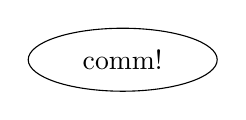
\begin{tikzpicture}\draw (0,0) ellipse (1.2 and .4);\node at (0,0) {comm!};\end{tikzpicture}}}&\\
\mathcal E\arrow[rr,"T_{-U}"']&&\mathcal E
\end{tikzcd}}
\[
 b'=b\deleted{\unsure{i}}\unsure{+|-}\chi U
\]
\[
 U-\gamma b'=U-\gamma b\unsure{-|+}\gamma\chi U=-U-\gamma b
\]
car
\figure{\begin{tikzpicture}\draw (0,.5) .. controls (0,.2) and (-.4,.1) .. (-.4,-.2);\end{tikzpicture}}

d'où un iso d'ext. $\chi$-\unsure{scindées}
\[
 E_1\vee E_2\simeq E_1\wedge E_2
\]
\[
 E'_1\vee E'_2\simeq E'_1\wedge E'_2
\]
\unsure{Je dis qu'il est fonctoriel pour les} \uuline{iso}) : c'est clair par construction.
Mais il y a aussi une notion d'\uuline{hom} d'ext. $\chi$-\unsure{scindées}. Ça marche aussi
\diagram{\begin{tikzcd}[column sep=small,row sep=small]
&&&&\unsure{M'_i}\arrow[dd,no head]&&\\
&L_i\arrow[dl,equal]\arrow[rr,no head]&&E'_i\arrow[dl]\arrow[rr]&&M'_i\arrow[dl,Rightarrow]\arrow[dd,equal]\\
L_i\arrow[rr,no head]\arrow[dd,Rightarrow]&&E_i\arrow[rr,no head]\arrow[dd]&&M_i\arrow[dd,equal]&&\\
&L'_i\arrow[dl,equal]\arrow[rr,no head]&&\unsure{E^{\prime\prime\prime}_i}\arrow[dl,no head]\arrow[rr,no head]&&M'_i\arrow[dl]\\
L'_i\arrow[rr,no head]&&E''_i\arrow[rr,no head]&&M_i&&
\end{tikzcd}}
\diagram{\begin{tikzcd}[column sep=small,row sep=large]
&&M'_1\otimes M'_2\arrow[d,no head]\\
L_1\otimes L_2\arrow[r]\arrow[d,Rightarrow]&E\arrow[r,Rightarrow]&M_1\otimes M_2\\
L'_1\otimes L'_2&&
\end{tikzcd}}
\mspage{125}
